\chapter{Determinación de Velocidad de Giro en Propelas}\label{App:tracker}
\vspace{-1cm} Los efectos hidrodinámicos modifican la velocidad a la que las especies llegan a la interfaz de la membrana con las disoluciones y pueden añadir variabilidad a los resultados experimentales. Estos efectos están dictaminados por la forma geométrica de la celda y de la propela, el volumen de la disolución, la ubicación espacial de la propela al interior de la semicelda y principalmente, su rapidez de rotación.

La rapidez de giro de las propelas puede determinarse de manera precisa y rápida usando un tacómetro láser que mide el periodo de pulsos láser que son reflejados cada vez que un objeto en rotación completa una revolución. El uso de un tacómetro láser hace necesario fijar un adhesivo reflectivo en una de las paletas de la propela para permitir que la radiación del láser rebote hasta el detector del tacómetro. La necesidad del adhesivo reflectivo hace que la rapidez de giro de la propela no pueda medirse mientras ésta se encuentra sumergida en una disolución (i.e.\ durante un proceso de transporte) por riesgo a que el adhesivo se desprenda o peor aún, que contamine las muestras que se están estudiando. Se determinó que para determinar la rapidez de giro de las propelas sin añadir elementos extraños a estas puede usarse la cámara de un teléfono celular capaz de grabar videos en cámara lenta para posteriormente hacer uso de programas adecuados de procesamiento de datos en video. La capacidad del método depende de la frecuencia de obturación de la cámara, medida en \ac{FPS}.

La celda de transporte con las propelas en rotación se ubica frente a un fondo oscuro y se graba durante 10 segundos usando una cámara de alta velocidad (Dual Camera iPhone 7 plus, Apple. 240 \ac{FPS}) mientras se encuentra en operación. El vídeo resultante se analiza usando la herramienta de perfil puntual \ac{RGB} del programa Tracker creado por \citet{tracker}. La rapidez de rotación de ambas propelas puede determinarse usando el mismo video. 

Primero debe importarse el video a Tracker haciendo clic en \colorbox{lgray}{\texttt{File > Import > Video...}} y seleccionando el archivo correspondiente. Cuando carguen todas los fotogramas del video, la ventana de Tracker lucirá similar a como se muestra en la Figura \ref{fig:track0}.

\begin{figure}[H]
    \centering
        \begin{picture}(500,260)
            \put(0, 0){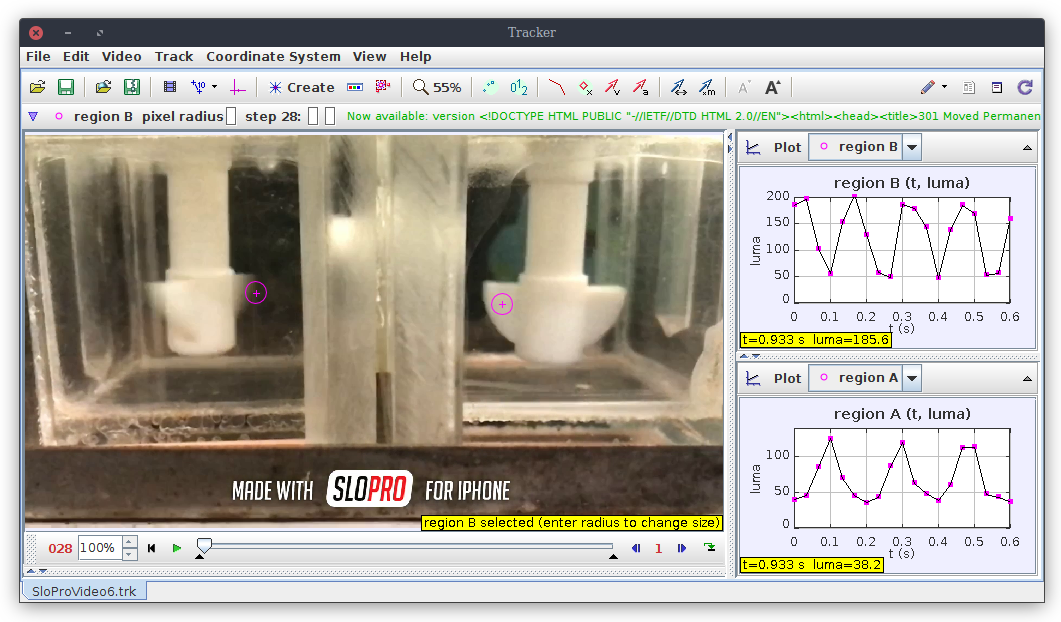
\includegraphics[width=\textwidth]{App/images/tracker.png}}
            \put(111, 145.5){\large\protect\starfvpointswht}
            \put(223, 139.5){\large\protect\starfvpointsblck}
            \put(339, 216.5){\Large\protect\circleblck}
            \put(339, 112){\Large\protect\circleblck}
            \put(410, 216.5){\Large\protect\squareblck}
            \put(410, 112){\Large\protect\squareblck}
        \end{picture}    
    \caption[Análisis del video de las propelas usando Tracker.]{Grabación del perfil \ac{RGB} en los puntos apropiados (\protect\starfvpointsblck) para determinar la rapidez de rotación de las propelas.}
    \label{fig:track0}
\end{figure}


Los puntos que se monitorean deben coincidir con regiones de la imagen en donde pasan las paletas de la propela. Para la creación de los perfiles \ac{RGB} se debe seleccionar \colorbox{lgray}{\texttt{Create > RGB Region}}. La posición del punto se marca haciendo clic en la región deseada mientras se sostiene la tecla \colorbox{lgray}{\texttt{Shift}}. Cuando se presiona el botón \colorbox{lgray}{\texttt{Play \trianglerigthblck}} en la región inferior de la ventana, Tracker empieza a grabar el perfil \ac{RGB} en cada punto y la información aparece en forma de tabla o de gráfico en la región derecha de la ventana.

La información de utilidad es la intensidad percibida (en unidades arbitrarias \textit{luma}). La intensidad percibida presenta un pico cada que la una de las aletas de la propela pasan por el punto de medición. Las propelas son simétricas y una revolución implica el paso de dos aletas por dicho punto. Los perfiles (uno por cada propela) deben exportarse como tablas de texto plano para su análisis. Para esto, debe cambiarse la representación de los resultados de modo gráfico a modo tabla, seleccionando en el esquema al lado izquierdo de \colorbox{lgray}{\texttt{Plot}} (marcado en la Figura \ref{fig:track0} con círculos negros) y seleccionando \colorbox{lgray}{\texttt{Table View}} en el menú desplegable. La información de ambos puntos (regiones A y B) debe aparecer en pantalla para que aparezcan disponibles en la ventana de exportación. Si solo una de las regiones aparece en ambas subventanas, la region faltante debe mostrarse haciendo clic en el menú desplegable marcado con un cuadrado negro en la Figura \ref{fig:track0} y seleccionando la región deseada. Para exportar las tablas de datos se hace clic en \colorbox{lgray}{\texttt{File > Export > Data File...}}. Se abre una ventana pequeña con cuatro menús desplegables donde se configura el archivo que va a ser generado. En \colorbox{lgray}{\texttt{Data Table}} se selecciona la región que se exportará y en \colorbox{lgray}{\texttt{Cells}} debe seleccionarse \colorbox{lgray}{\texttt{All Cells}}. En \colorbox{lgray}{\texttt{Delimiter}} lo más conveniente es seleccionar \colorbox{lgray}{\texttt{Comma}}. Al hacer clic en \colorbox{lgray}{\texttt{Save As...}} el archivo puede guardarse en la ubicación que se desee. El proceso de exportación debe hacerse de manera independiente para cada perfil RGB.

%\colorbox{lgray}{\texttt{}}

Los archivos generados se procesan usando \verb|R| \citep{R}. Las funciones se encargan de filtrar la información para eliminar ruido lumínico ambiental y cuentan el número de picos para obtener la rapidez de rotación usando la Ecuación  \ref{eq:propelas}.

\begin{equation}\label{eq:propelas}
    \Theta = \frac{Pck}{Ph}\cdot7200
\end{equation}
donde $\Theta$ es la rapidez de giro, en \ac{RPM}, $Pck$ es el número de picos contados, $Ph$ es el numero de fotogramas del video y 7200 es el factor requerido para convertir picos contados a revoluciones (2 picos por revolución), fotogramas a segundos (240 \ac{FPS}) y segundos a minutos.

Las funciones que se usan son las siguientes:
\begin{lstlisting}[belowskip=-2.6\baselineskip]
find_peaks <- function (x, m = 3) { ## source: https://github.com/stas-g/findPeaks
  shape <- diff(sign(diff(x, na.pad = FALSE)))
  pks <- sapply(which(shape < 0), FUN = function(i) {
    z <- i - m + 1
    z <- ifelse(z > 0, z, 1)
    w <- i + m + 1
    w <- ifelse(w < length(x), w, length(x))
    if (all(x[c(z:i, (i + 2):w)] <= x[i + 1])) {
      return(i + 1)
    } else {
      return(numeric(0))
    } 
  })
  return(unlist(pks))
}

RobustRPM <- function (lum, fps = 240, n = 50, frac = 10, m = 3, plot = TRUE) {
  ngr <- trunc(length(lum) / frac)
  X <- vector()
  for (i in 1:frac) {
    lumi <- lum[((i - 1) * ngr + 1):(i * ngr)]
    peaks <- find_peaks(x = lumi, m = m)
    rev = length(peaks) / 2
    time = length(lumi) / 240 / 60
    X <- c(X, rev / time)
  }
  
  if (plot) {
    plot(lumi, xlim = c(1, n), type = 'o', xlab = 'Fotograma', ylab = 'Luminancia (lumas)')
    points(x = peaks, y = lumi[peaks], col = 2, pch = 8)
  }
  cat('Rapidez de rotacion:', trunc(mean(X), 0), '+-', trunc(2 * sd(X), 0), 'RPM')
  #return(X)
}
\end{lstlisting}

El uso de las funciones para obtener el resultado se muestra a continuación:
\begin{lstlisting}[belowskip=-2.6\baselineskip]
## Cargamos los datos y visualizamos las primeras filas:
data <- read.table("example_1192", skip = 1, header = TRUE, sep = ',')
head(data, n = 10)
#      >            t        x        y      luma
#      > 1 0.00000000 -213.3333  5.824801  54.18125
#      > 2 0.03333333 -201.6837 -2.912400  39.82353
#      > 3 0.06666667 -201.6837 -2.912400  48.86556
#      > 4 0.10000000 -201.6837 -2.912400  92.62610
#      > 5 0.13333333 -201.6837 -2.912400 154.28881
#      > 6 0.16666667 -201.6837 -2.912400  99.63448

## Corremos la funcion usando la columna que tiene los datos de luminancia:
RobustRPM(lum = data$luma, fps = 240, frac = 10, n = 50, m = 3, plot = TRUE)
#      > Rapidez de rotacion: 1192 +- 16 RPM. (95% de confianza)
\end{lstlisting}

Aparte del resultado numérico con incertidumbre, se produce el gráfico de luminancia percibida en función del fotograma para valores hasta \verb|(n = 50)| como se muestra en la Figura \ref{fig:tracker}(a). El gráfico marca los puntos que fueron seleccionados como picos en el conjunto de datos ingresado. Esto permite verificar que oscilaciones en el ruido lumínico ambiental no sean contados como giros de la propela al presentar falsos máximos como podría observarse en la Figura \ref{fig:tracker}(b). 

\begin{figure}[H]
\centering
    \subbottom{\begin{picture}(245,145)
               \put(-1.7, 0){\includegraphics[height=0.31\textwidth, page = 2]{App/images/Tracker.pdf}}
               \put(31, 129){\large a)}
                \end{picture}}%
    \subbottom{\begin{picture}(225,117)
               \put(0, 0){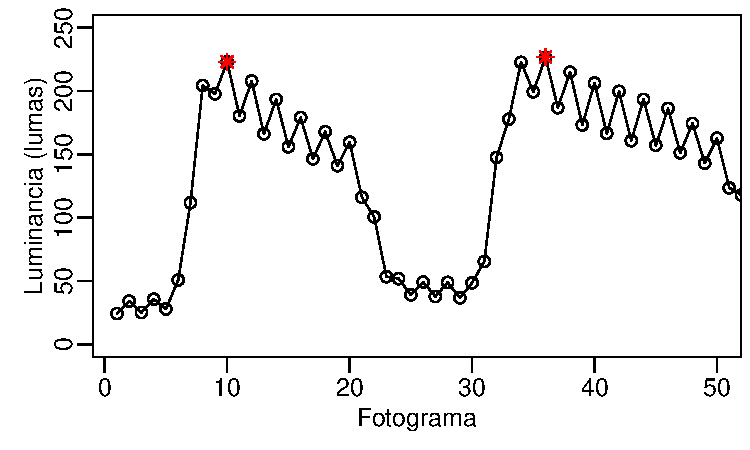
\includegraphics[height=0.31\textwidth, page = 1, trim = {1.45cm 0 0 0},   clip]{App/images/Tracker.pdf}}
               \put(6, 129){\large b)}
               \end{picture}}%
    \caption[Luminancia en función del fotograma para determinar rapidez de giro de propela.]{Luminancia en función del fotograma para propelas girando a a) 1192$\pm$ 16 y a b) 290$\pm$17 RPM.}
    \label{fig:tracker}
\end{figure} 

El método permite medir valores de rapidez de rotación de más de 1500 RPM. Este valor solo se encuentra limitado por la frecuencia máxima de obturación de la cámara de alta velocidad. El procesamiento del video en Tracker consume una cantidad apreciable de recursos del procesador por lo que se recomienda no tener muchos programas abiertos en la computadora al momento de hacerlo.

\ChapBib{App/App}